\documentclass{article}

\usepackage{assign}
\setcoursetitle{Algorithms II}
\setassigncode{4}
\setauthname{Gurpreet Singh, Nikita Awasthi}
\setauthroll{150259, 150453}

\begin{document}
\makeheader%

\begin{question}

	Given a sequence of graphs $G_0$, $G_1$, \dots, $G_b$ such that all the graphs are connected, we need to minimize

	\begin{align*}
		cost(P_0, P_1, \dots , P_b) &= \sum_{i=0}^b l(P_i) + K.changes(P_0, P_1, \dots, P_b) 
	\end{align*}

	where $changes(P_0, P_1, \dots, P_b)$ is the number of indices such that $0 \leq i < b$ and $P_i \neq P_{i+1}$

	\begin{qsection}{Pseudocode}

		The algorithm is given on the next page

		\begin{algorithm}[h!]
			\begin{algorithmic}[1]
            	\caption{Computing minimum cost}
                \Procedure{MinimumCost}{${G_0, G_1, \dots, G_b}, b, K$} \Comment{where K is the constant }
                    \For{$0 \le i \le b$}
						\State{$G(i, i) = G_i$}
                        \For{$ i < j \le b$} 
							\State{$G(i,j) = G(i, j - 1) \cap G_j$} \\
                            \Comment{where $G(i,j)$ is the graph containing the edges which are common between all graphs $G_i \dots G_j$}
							\\
							\State{Compute $l(i,j)$ and $P(i,j)$} \\
							\Comment{$l(i,j)$ is the length of the shortest s-t path $P(i,j)$ in $G(i,j)$, if it exists, otherwise $l(i,j) = \infty$}
                        \EndFor%
                    \EndFor%
					\\
                    \For{$0 \leq i \leq b$}
						\State{$DP[i] = (i+1) \cdot \func{l}{0, i}$}
						\State{$SP[i] = -1$}
						\Comment{$SP[i]$ stores the last path split/change point for optimal paths for Graphs 0 to $i$}
						\\
                        \For{$1 \leq j < i$}
							\If{$DP[i] > DP[j] + K + (i - j) \cdot \func{l}{j + 1, i}$}
								\State{$DP[i] = DP[j] + K + (i - j) \cdot \func{l}{j + 1, i}$}
								\State{$SP[i] = j$}
							\EndIf%
                        \EndFor%
                    \EndFor%
					\\
                    \State{$i=b$}
                    \While{$i \geq 0$}
                        \If{$SP[i] == -1$}
                            \State{$P[0 \dots i] = P(0,i)$}
                            \State{$i=-1$}
                        \Else%
							\State{$j = SP[i]$}
                            \State{$P[j \dots i]=P(j,i)$}
                            \State{$i = j-1$}
                        \EndIf%
                    \EndWhile%
                \EndProcedure%
            \end{algorithmic}
		\end{algorithm}
	\end{qsection}
	
	\begin{qsection}{Proof of Correctness}
		The notations used in the algorithm are as follows:

		\begin{enumerate}
			\item $G(i,j)$ is constructed using the graphs $G_i, \dots G_j$ containing all the vertices. However, the edges in the resultant graph are those which are common to all the graphs.
			\item $l(i,j)$ and $P(i,j)$ represents the length of the shortest path and the shortest path between s and t in $G(i,j)$. This is computed using BFS traversal of the graph.
			\item $DP[i]$ represents the optimal value of the cost when considering the graphs $G_0, \dots , G_i$ corresponding to the optimal set of paths $P_0, \dots , P_i$.
			\item $SP[i]$ represents the last point where path is different when considering the graphs $G_0, \dots , G_i$.
		\end{enumerate}

		\begin{qsubsection}{Proof of Sub-Optimal Property}

			If there is no path change, then there is no sub-problem and this case is trivial. However, if there is at least one path change, consider the last path change, say at index $j$. Now, we have two sub-problems, one is the trivial case, \textit{i.e.} the paths from $j + 1$ to $b$, and another is the paths from $0$ to $j$. Since the cost of these sub-problems is directly added and is independent, we can claim that both the sub-problems must be optimal. And hence, the sub-optimal property exists.
			
		\end{qsubsection}

		\begin{qsubsection}{Proof of recurrence}

			Given that all the graphs are connected, there will always exist an s-t path in any of the graphs $G_0, \dots, G_b$. To compute the optimal solution and the cost associated with it for a graphs $G_0, \dots, G_b$, we can consider any arbitrary $i$ s.t $0 \leq i \leq b$. Now there are two cases possible \br%

			\begin{qcase}{1}{There is no change in the paths $P_0, \dots, P_i$}
				If there is no change in the paths $P_0, \dots , P_i$, then the $cost(P_0, \dots , P_i) = \sum_{j=0}^i l(j)$. \br%
				
				Since there is no change, all the paths would be the same and the combined graph $G(0,i)$ will have all the edges of $P_0$ which would essentially be $P(0,i)$ and its length $l(0,i)$.
			\end{qcase}

			\begin{qcase}{2}{There is at least one change in the paths $P_0, \dots, P_i$}
				There is a change in path at an index before i. Let us consider j to be the largest index such that change occurs between graphs $G_j$ and $G_{j+1}$. In such a case, there would be no change between graphs $G_{j+1}, \dots, G_i$ and $cost(P_0, \dots , P_i)= cost(P_0, \dots , P_j) + (i-j)l(j+1,i) + K$ where the K term accounts for the change $G_j$ and $G_{j+1}$
			\end{qcase}

			As a result, the recurrence for the minimum cost represented by $DP[b]$ reduces to 

			\begin{align*}
				DP[b] &= \min((b+1)l(0,b), \min_{0 \leq i \leq b}(DP[i] + (b-i) \, \func{l}{i + 1, b} + K))
			\end{align*}

			\textbf{Base Case:} For the base case of $b=0$, $DP[0] = l(0, 0)$ which is the length of the shortest s-t path in $G_0$ corresponding to which we would have $P_0 = P(0, 0)$. This is consistent with our definition and our algorithm.
		\end{qsubsection}

	\end{qsection}

	\clearpage

	\begin{qsection}{Time Complexity}

		\begin{qsubsection}{Pre-Processing}

			Pre-processing consists of computing $G(i,j)$ along with $l(i,j)$ and $P(i,j)$. In order to compute the intersection graph, we simply need to loop through all the vertices and edges \textit{i.e.} $\bigO{n + m}$. For finding the shortest path and it's length, we use BFS traversal for this purpose which is again $\bigO{m + n}$.

			Since we need to compute for all pairs, which is $b^2$, the total preprocessing time is $\bigP{(m + n)b^2}$.

		\end{qsubsection}

		\begin{qsubsection}{Final Computation}
			
			For every index $i$ from 0 to $b$, an inner loop with variable $j$ varies from $1$ to $i$. This leads to an $O(b^2)$ time complexity to find the optimal path sequence with associated minimum cost.

		\end{qsubsection}
		
	\end{qsection}

\end{question}

\begin{question}

	Consider the distance between the source $s$ and the sink $t$ to be $\ge k \cdot n^{2/3}$ for some constant $k > 0$. For the rest of this question, let $r = k \cdot n^{2/3}$ \br%

	From the complexity analysis of Ford-Fulkerson Algorithm, we know the that it takes $O(mf)$ time, where $f$ is the max-flow. Also, we know that this flow is equal to the capacity of the minimum capacity cut for the max-flow graph. \br%

	Assume that for the given graph, the flow $f$ is not bounded by $\bigO{n^{2/3}}$ \textit{i.e.} $f \notin \bigO{n^{2/3}}$. Hence the capacity of any cut will not be bounded by $\bigO{n^{2/3}}$. \br%

	If we start from the cut with only the source vertex, and iteratively add the vertices that are connected to this cut by an edge. Let this set of vertices to be added be $V_i$. This can also be defined as the set of vertices at a distance $i$ from the source vertex $s$. Also, $V_0 = \set{s}$ \br%

	We only consider for $i < r$ as after that, we will be considering the sink vertex which is not desired. From the set of vertices, we can trivially say $V_0 \cup V_1 \dots \cup V_{r - 1} \subset V(G)$. Hence,

	\begin{align*}
		\abs{V_0} + \abs{V_1} \,\dots\, \abs{V_{r - 1}}	&\qlt	n \\
		\shortintertext{Using AP-GP rule}
		\abs{V_1} \abs{V_2} \,\dots\, \abs{V_{r - 1}}	&\qlt	\para{\frac{n}{r}}^{r - 1}
	\end{align*}

	However, since the capacity of each cut must be greater than $r$, hence the number of out edges must be greater than $r$. Thus, we can say $\abs{V_i} \abs{V_{i + 1}} > r$, since number of out edges $< \abs{V_i} \abs{V_{i + 1}}$. Therefore, we can write

	\begin{align*}
		\abs{V_1} \abs{V_2} \abs{V_3} \dots \abs{V_{r - 1}}	\qgt	\para{\frac{n}{r}}^{r - 1}
	\end{align*}

	However, this is a contradiction. Hence, the capacity of the minimum capacity cut must be bounded by $\bigO{n^{2/3}}$ and thereby, the flow is bounded by $\bigO{n^{2/3}}$. Thus, the time taken by the Ford-Fulkerson algorithm is bounded by $\bigO{mn^{2/3}}$.

\end{question}

\begin{question}
	
	\begin{qpart}{1}

		We can transform this problem to an instance of the Max-Flow problem with lower bound on edge capacities (discussed in class).

		\begin{qsection}{Pseudocode}

			The construction of the graph for the Max-Flow instance is as follows

			\begin{enumerate}
				\item Create a node $B_i$ for each balloon $i \in [m]$ and a node $C_j$ for each condition $j \in [n]$
				\item Create a source vertex $S$, and connect $S$ to each node $B_i$ (for all $i \in [m]$) with upper edge capacity 2 and lower edge capacity 0
				\item Create a sink vertex $T$, and connect each node $C_j$ (for all $j \in [n]$) to $T$ with upper edge capacity $\infty$ and lower edge capacity $k$ 
				\item For each node $B_i$, connect $B_i$ to $C_j$, if $C_j \in S_i$, with upper edge capacity 1 and lower edge capacity 0
			\end{enumerate}

			\begin{figure}[h!]
				\centering
				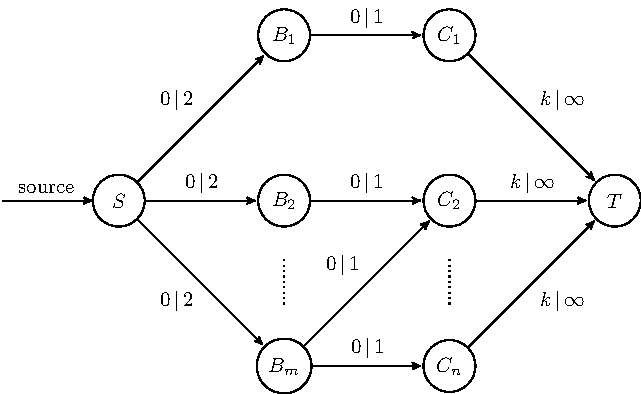
\includegraphics{q1-max-flow-instance.pdf}
				\caption{An illustration of the converted instance of the Max-Flow problem}
			\end{figure}

			After this, compute an integral max flow (or any flow) for this instance using the algorithm discussed in class. If such a flow exists, we return \textit{TRUE}, else we return \textit{FALSE}. If we need to report which balloon must check which condition, we need to consider an integral flow. Then for each balloon $i$, $B_i$ can be connected to at most two nodes from the set of condition nodes \textit{i.e.} $\set{C_j}_{j = 1}^{n}$, we can simply report these conditions for this balloon.

		\end{qsection}

		\begin{qsection}{Proof of Correctness}

			\begin{qproof}{If there exists a configuration or mapping of the balloons, such that this mapping follows all the constraints, then we can construct a flow for the same instance constructed above}

				We have a mapping from each balloon $i$ to at most two conditions. For each condition $j$, mark the flow on the edge $\para{B_i, C_j} = 1$, and mark the flow on the edge $\para{S, B_i}$ equal to the number of conditions the balloon $B_i$ is mapped to. Also, for each edge $C_j, T$, mark the flow equal to the number of balloons such that $C_j$ is in the mapping for those balloons. \br%

				We can show that this is a valid flow, and follows all constraints of the constructed Max-Flow graph. \br%

				\begin{qsubsection}{Capacity Constraint}

					For all edges $\para{S, B_i}$, the lower bound constraint is trivially satisfied. Since each balloon is mapped to at most two conditions, therefore we cannot have the flow for this edge to be greater than 2. Hence, the constraint for all such edges is followed. \br%

					For all edges $\para{C_j, T}$, the upper bound constraint is trivially satisfied. Since the mapping is valid and follows the constraint of minimum number of balloons for each condition as $k$. Therefore, each condition will be in the mapping from at least $k$ balloons, and hence the lower bound constraint is also satisfied. \br%

					For all edges $\para{B_i, C_j}$, both the lower and upper bound constraints are satisfied, as we only assign 1 or 0 flow to each edge.

				\end{qsubsection}

				\begin{qsubsection}{Conservation Constraint}

					For each balloon $i$, we know that the number of edges $\para{B_i, C_j}$ which have 1 flow will be the flow for the edge $\para{S, B_i}$. Hence the flow is conserved at each node $B_i$. \br%

					For each condition $j$, we know that the number of edges $\para{B_i, C_j}$ which have 1 flow will be the flow for the edge $\para{C_j, T}$. Hence the flow is conserved at each node $C_j$.

				\end{qsubsection}

				Since all constraints are satisfied, we have a valid flow. Hence our claim is true.

			\end{qproof}

			\begin{qproof}{If there exists a flow for the given construction, then there exists a mapping from a balloon to at most two conditions which satisfies all the constraints in the question}

				Using the integrality of flow (discussed in class), we can say there exists an integral flow. Hence, for each edge $\para{B_i, C_j}$, the flow is either 0 or 1. \br%

				Since the edge capacity for all edges $\para{S, B_i}$ is 2, there can be only two edges for each balloon $i$, such that the flow through $\para{B_i, C_j}$ is 1. For each such edge, add a mapping from balloon $i$ to condition $j$. The constraint that one balloon must be mapped to at most 2 conditions is, thus, satisfied. \br%

				Also, since the minimum flow through each edge $\para{C_j, T}$ must be at least $k$, hence, we can say that for each condition $C_j$, there must be at least $k$ edges such that the flow through $\para{B_i, C_j}$ is 1. Therefore, each condition $C_j$ is in at least $k$ mappings, thus, satisfying all constraints. \br%

				Hence, if there exists a valid flow, we can find a valid mapping.

			\end{qproof}

			Using the above two claims, we can say that solving the constructed Max-Flow problem is the same as solving the original question. Hence our algorithm is correct.

		\end{qsection}

	\end{qpart}

	\begin{qpart}{2}

		We only need to change the construction of the Max-Flow Problem to satisfy the additional constraints.

		\begin{enumerate}
			\item Create a node $B_i$ for each balloon $i \in [m]$, a node $C_j$ for each condition $j \in [n]$ and a node $SC_l$ for each sub-contractor $l \in [3]$
			\item Create a source vertex $S$, and connect $S$ to each node $SC_l$ (for all $l \in [3]$) with upper edge capacity $\infty$ and lower edge capacity $k$
			\item Connect each node $SC_l$ to each node $C_j$ (for all $l \in [3]$ and $j \in [n]$) with upper edge capacity $k - 1$ and lower edge capacity $0$
			\item Create dummy nodes $\pr{C}_j$ (for all $j \in [l]$) and connect $C_j$ to $\pr{C}_j$ with upper edge capacity $\infty$ and lower edge capacity $k$
			\item For each $B_i$, connect $\pr{C}_j$ to $B_i$, if $j \in S_i$, with upper edge capacity 1 and lower edge capacity 0
			\item Create a sink vertex $T$, and connect each node $B_i$ (for all $i \in [m]$) to $T$ with upper edge capacity 2 and lower edge capacity 0
		\end{enumerate}

		After this, we can proceed as we did in the first part.
		
	\end{qpart}

\end{question}

\end{document}
